\section{Jednoosobowy serniczek ciasteczkowy}
\bigskip
\small
\begin{minipage}{0.45\textwidth}
    \noindent \textbf{Czas:} 60 minut \\
    \textbf{Poziom trudności:} łatwy
\end{minipage}
\begin{minipage}{0.45\textwidth}
    \noindent \textbf{Ilość sprzątania:} średnia\\
    \textbf{Wymagany mysi sprzęt:} Mini foremka do ciasta lub ramekin
\end{minipage}
\normalsize
\vspace{0.5cm}

\begin{multicols}{2}

\subsection*{Składniki}
\begin{itemize}
    \item 2 garści ulubionych kruchych ciasteczek
    \item 3-4 duże łyżki masła
    \item 2 łyżki śmietankowego serka kanapkowego (najlepiej takiego bez soli) lub serka mascarpone
    \item 0.5 opakowania lekkiego serka typu ,,Bieluch"
    \item 2 łyżki ulubionego kremu (np. Nutella, masło orzechowe, krem ciasteczkowy Biscoff lub karmel)
    \item 1 płaska łyżka cukru pudru (opcjonalnie)
\end{itemize}

\columnbreak

\begin{figure}[H]
    \centering
    \fbox{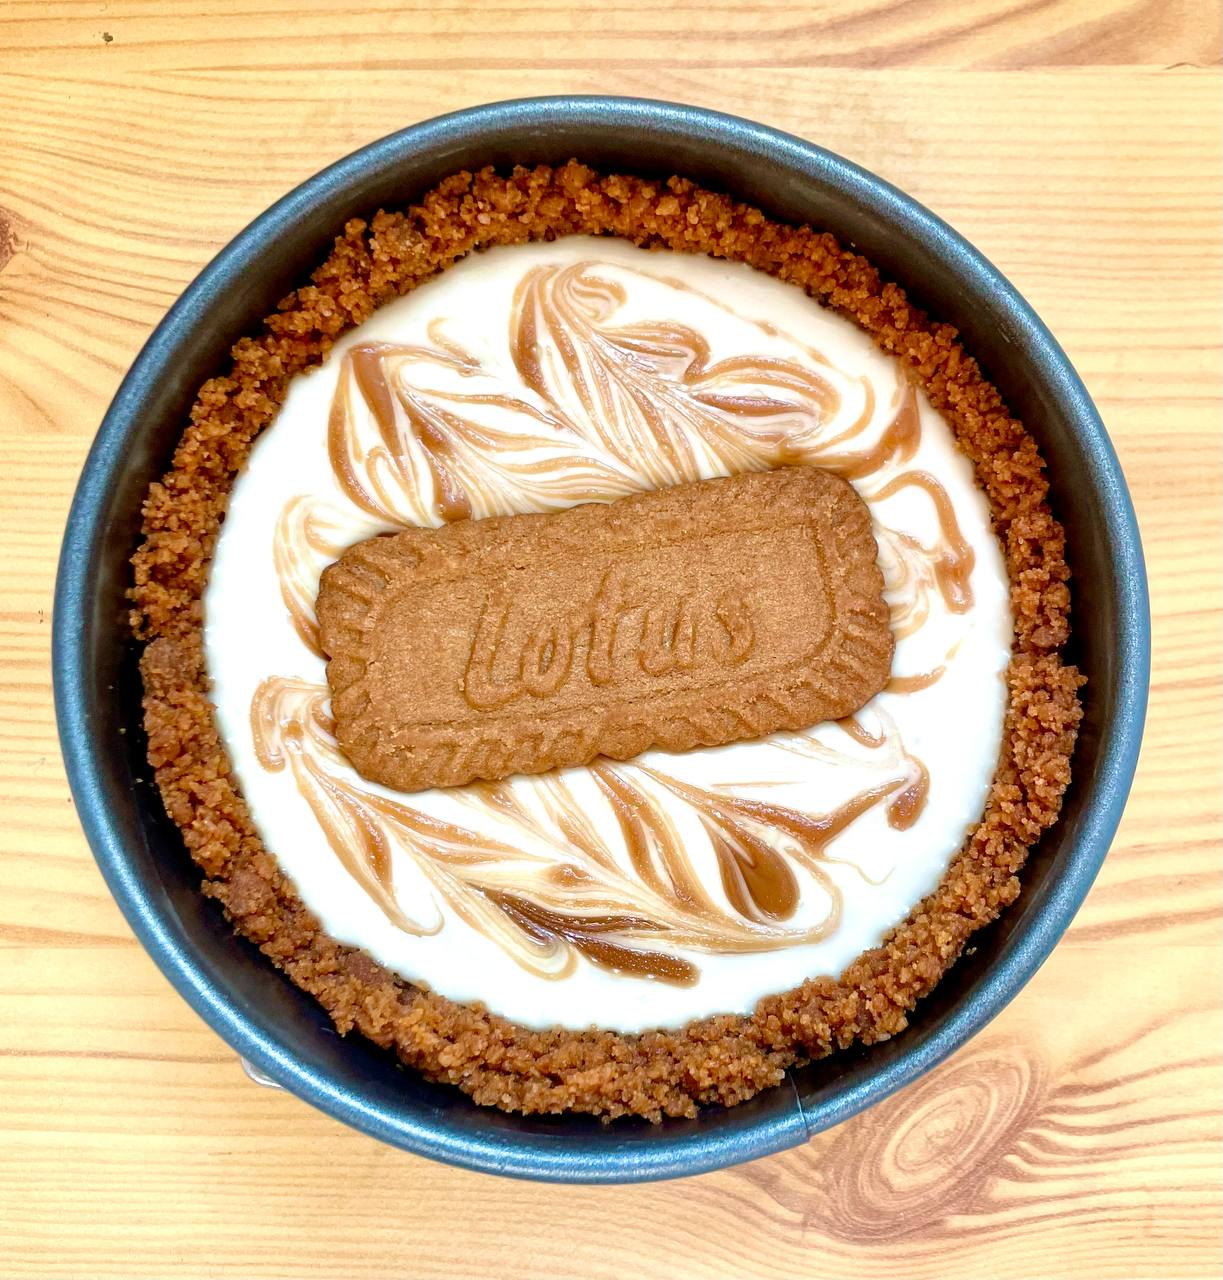
\includegraphics[width=0.35\textwidth]{images/serniczek.jpg}}
\end{figure}
\end{multicols}

\vspace{0.5cm}

\subsection*{Instruktaż}
\begin{enumerate}
    \item Ciasteczka włożyć do woreczka strunowego i pokruszyć na drobno czymś ciężkim, np wałkiem lub niewielką patelnią. Pyłek przełożyć do miski i zalać roztopionym masłem do uzyskania konsystencji mokrego piasku. Przesypać do foremki, uklepać mocno na dnie i ewentualnie odrobinę na ściankach, najlepiej łyżką lub szklanką o płaskim dnie. Wstawić do lodówki na 10-15 minut.
    \item Pozostałe składniki wymieszać w misce do uzyskania jednolitej konsystencji i przełożyć na utwardzony spód. Całość schłodzić w lodówce na około 45 minut lub aż do stężenia masy.
\end{enumerate}

\vspace{0.5cm}

\small
\subsection*{Propozycja podania}
Z dekoracją z ciasteczek.

\vspace{0.3cm}

\subsection*{Dodatkowe uwagi}
Czas stężenia masy może różnić się w zależności od wielkości foremki i ilości masy.

\newpage
